\section{Results}

\subsection{Requirements Check}

\begin{table}[H]
\centering
\caption{Requirement verification in the closed-loop 6DOF simulation.}
\begin{tabular}{p{0.28\textwidth}p{0.20\textwidth}p{0.34\textwidth}c}
\toprule
Criterion & Required & Obtained & Status \\
\midrule
Bingo (hits target) & miss $<20~\text{m}$ & $17.9~\text{m}$, Mach $0.90$, $207~\text{s}$ & Satisfied \\
Terminal maneuver & $\geq 5g$ & $\approx 5.6g$ (Gmax $2\rightarrow 7.4g$) & Satisfied \\
Airframe bandwidth & $\geq 0.5~\text{Hz}$ & attitude $2.6$--$3.6~\text{Hz}$, accel $0.7$--$1.3~\text{Hz}$ & Satisfied \\
Trim (all CG phases) & within $\pm 20^\circ$ & launch $-18^\circ$ \ldots terminal $-12^\circ$ & Satisfied \\
Follow command & $\text{DC}=1$, stable & $\text{DC}=1.00$, damped & Satisfied \\
Cruise held & Mach $0.90$ & sustainer holds (thrust $=$ trim drag) & Satisfied \\
\bottomrule
\end{tabular}
\end{table}

\subsection{Homing Flight}

The horizontal trajectory reaches the target, the altitude profile is sea-skimming ($\approx 26~\text{m}$), and the speed holds cruise. The miss distance is $17.9~\text{m}<20~\text{m}$, so the fuze detonates (BINGO). With the target nearly ahead, the LOS rate is small, so the terminal maneuver is small and the run is almost straight, with the boresight error tending to zero at impact.

\begin{figure}[H]
\centering
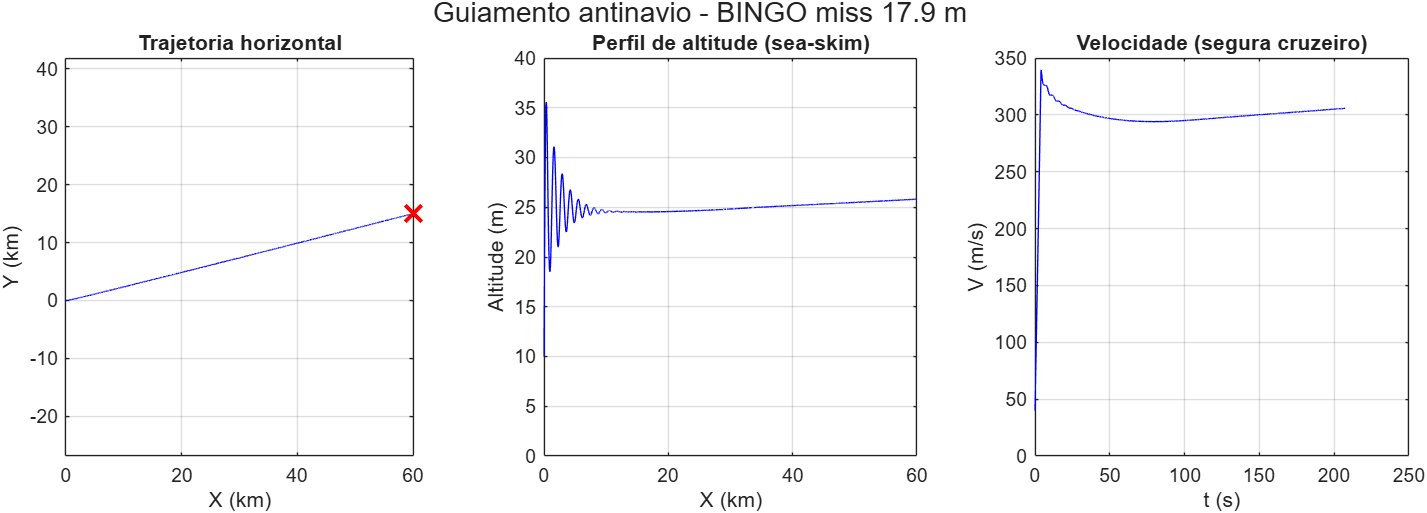
\includegraphics[width=0.92\textwidth]{figures/homing_trajectory.png}
\caption{Homing trajectory to bingo (horizontal trajectory, altitude profile and speed).}
\end{figure}

\begin{figure}[H]
\centering
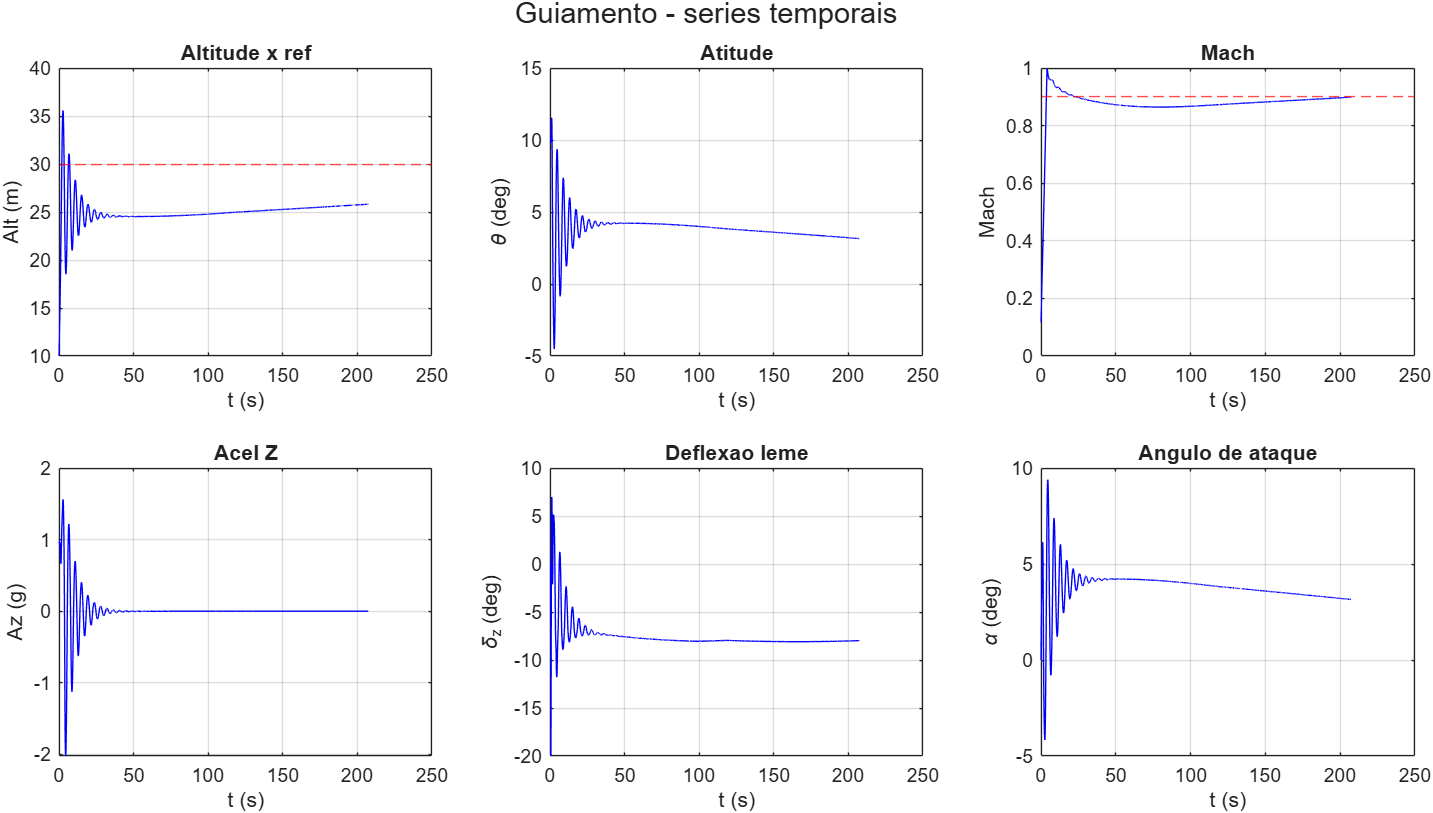
\includegraphics[width=0.92\textwidth]{figures/homing_series.png}
\caption{Flight time series: altitude versus reference, attitude $\theta$, Mach, acceleration $A_z$, fin deflection $\delta$ and angle of attack $\alpha$.}
\end{figure}

The flight phases are: boost $0$--$4~\text{s}$ ($0\rightarrow$ Mach $0.93$); transient $0$--$40~\text{s}$ (gains extrapolate below Mach $0.6$); smooth cruise $40$--$207~\text{s}$; and terminal to bingo at $207~\text{s}$.

\subsection{Engagement Envelope}

The envelope analysis (\texttt{Envelope6DOF.m}) sweeps launch positions and marks where the missile scores a bingo. Coverage is nearly omnidirectional (azimuths $0^\circ$--$150^\circ$), with a maximum range of $\approx 72$--$76~\text{km}>70~\text{km}$, limited by the sustainer burn ($\approx 232~\text{s}$). The missile fails only from directly behind ($180^\circ$), as expected for an antiship weapon.

\begin{figure}[H]
\centering
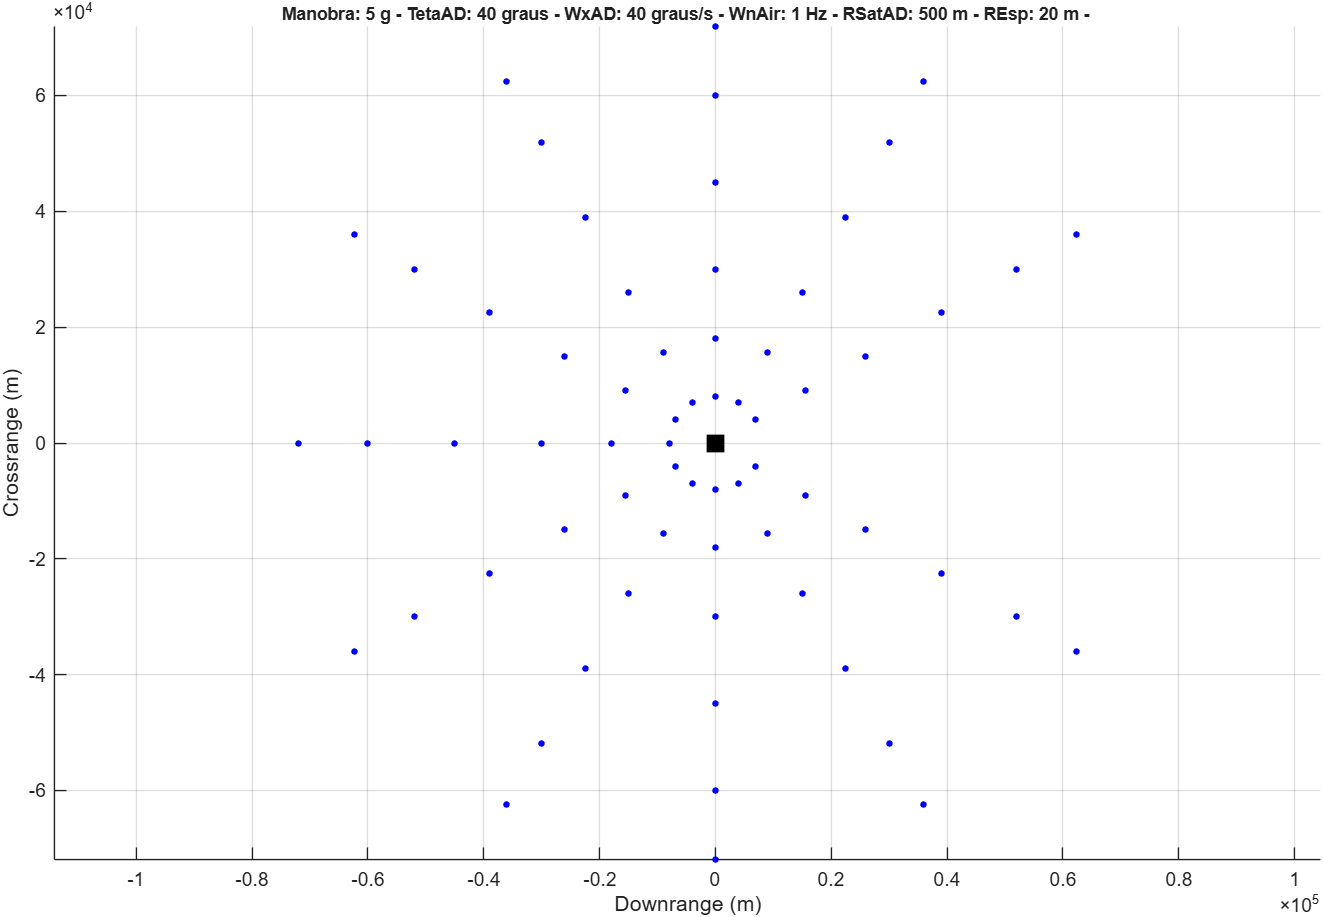
\includegraphics[width=0.72\textwidth]{figures/envelope.png}
\caption{Engagement envelope (downrange versus crossrange, ship at the origin).}
\end{figure}

A bug was found during this validation: the pre-programmed cruise heading \texttt{C.Rumo0} was computed once (from the initial geometry) and stayed effectively at $0^\circ$. Beyond $\approx 40^\circ$ launch azimuth the missile crossed to the wrong side and the seeker could not recover, producing false ``misses''. The fix is to recompute \texttt{Rumo0} from each launch geometry inside the loop, which corrected the whole envelope.
